\documentclass[11pt,a4paper]{article}
\author{TalentSprint}
\date{}
\usepackage{graphicx}
\usepackage{verbatim}
\usepackage{array}
\usepackage{caption}
\usepackage{enumitem}
\usepackage{xcolor}
\usepackage[tikz]{bclogo}
\usepackage{textcomp}
\usepackage{listings}
\usepackage{multicol}
\usepackage{float}
\usepackage{seqsplit} 
\usepackage{setspace}
\usepackage{soul}
\usepackage{latexsym}
\lstset{language=Java,numbers=left, numberstyle=\tiny, numbersep=10pt, showstringspaces=false, breaklines=true,keepspaces=true, columns=flexible}
\usepackage{fancyhdr}
\headheight=14pt
\lhead{\nouppercase{}}
\rhead{\nouppercase{\leftmark}}

\graphicspath{{../Images/}}


\begin{comment}
\setcounter{tocdepth}{1}
\setlength\parindent{0pt}
\parskip=4pt
\def\AnswerBox{\fbox{\begin{minipage}{4in}\hfill\vspace{0.5in}\end {minipage}}}

\thispagestyle{empty}
\vspace{1.5pc}
\topskip0pt
\vspace*{\fill}
\centerline{\sc \Huge Version Control System}
\vspace{2pc}
\vspace*{\fill}
\centerline{Prepared by TalentSprint WISE Team} 
\setcounter{page}{1}
\pagestyle{fancy}
\end{comment}


%========================================================================

% Lengths and widths
\addtolength{\textwidth}{2.5cm}
\addtolength{\hoffset}{0cm}
\setlength{\headsep}{-12pt} % Reduce space between header and content
\setlength{\headheight}{85pt} % If less, LaTeX automatically increases it
\renewcommand{\footrulewidth}{2pt} % Remove footer line
\renewcommand{\headrulewidth}{1pt} % Remove header line
\renewcommand{\seqinsert}{\ifmmode\allowbreak\else\-\fi} % Hyphens in seqsplit
% This two commands together give roughly
% the right line height in the tables
\renewcommand{\arraystretch}{1.3}
\onehalfspacing



% Commands
\newcommand{\SetRowColor}[1]{\noalign{\gdef\RowColorName{#1}}\rowcolor{\RowColorName}} % Shortcut for row colour
\newcommand{\mymulticolumn}[3]{\multicolumn{#1}{>{\columncolor{white}}#2}{#3}} % For coloured multi-cols
\newcolumntype{x}[1]{>{\raggedright}p{#1}} % New column types for ragged-right paragraph columns
\newcommand{\tn}{\tabularnewline} % Required as custom column type in use

% Font and Colours
\definecolor{HeadBackground}{HTML}{333333}
\definecolor{FootBackground}{HTML}{666666}
\definecolor{TextColor}{HTML}{333333}
\definecolor{DarkBackground}{HTML}{6B8E23} %{FD1AA8}
\definecolor{LightBackground}{HTML}{E8FED8} %D3FDC8
\definecolor{tit}{HTML}{FF6600}
\renewcommand{\familydefault}{\sfdefault}
\color{TextColor}
 \headsep = 25pt
% Header and Footer
\pagestyle{fancy}
\usepackage[headheight=110pt]{geometry}
\fancyhf{}% Clear header/footer

\fancyhead[r]{
\includegraphics[width = 4cm, height = 2cm]{TS-Logo.png}\hspace{0cm}}

%=================================TITLE=====================================
\fancyhead[l]{{\bf{\textcolor{tit}{\textrm{\large{Test Driven Development(TDD) and JUnit}}}}}}
%===========================================================================

\renewcommand{\headrulewidth}{0.4pt}% Default \headrulewidth is 0.4pt
\renewcommand{\footrulewidth}{0.4pt}% Default \footrulewidth is 0pt

\rfoot{Page \thepage}
\lfoot{COPYRIGHT \textcopyright TALENTSPRINT, 2015. ALL RIGHTS RESERVED.}


\begin{document}

\section*{TDD}
\subsection*{Origin}
Test Driven Development is a core part of agile process formalized by Kent Beck called eXtreme Programming(XP)

XP originally had the rule to test everything that could possibly break. Now, however, the practice of testing in XP has evolved into Test-Driven Development.

\subsection*{What is TDD?}

Test-driven development (TDD) is a software development process that relies on the repetition of a very short development cycle: first the developer writes an (initially failing) automated test case that defines a desired improvement or new function, then produces the minimum amount of code to pass that test, and finally refactors the new code to acceptable standards.

\subsection*{What can be tested?}
\begin{itemize}
\item Valid Input.
\item In-valid Input.
\item Exceptions.
\item Boundary conditions.
\item Everything that should be a possible break.
\end{itemize}

\subsection*{Aspects of TDD}
\begin{itemize}
\item Features.
\begin{itemize}
\item High level user requirements.
\item User story.
\end{itemize}
\item Customer Tests.
\begin{itemize}
\item Customer Identified user acceptance tests.
\end{itemize}
\item Developer Tests.
\begin{itemize}
\item Tests developed during software construction.
\end{itemize}
\end{itemize}

\subsection*{TDD life cycle}
The different steps involved in a test driven development cycle are:
\begin{itemize}
\item Write a single test.
\item Compile it. It shouldn't compile because you've not written the implementation code.
\item Implement just enough code to get the test to compile.
\item Implement just enough code to get the test to pass.
\item Run the test and see it pass.
\item Refactor for clarity.
\item Repeat.
\end{itemize}
\vfill{\ }
\begin{figure}[H]
 \begin{center}
   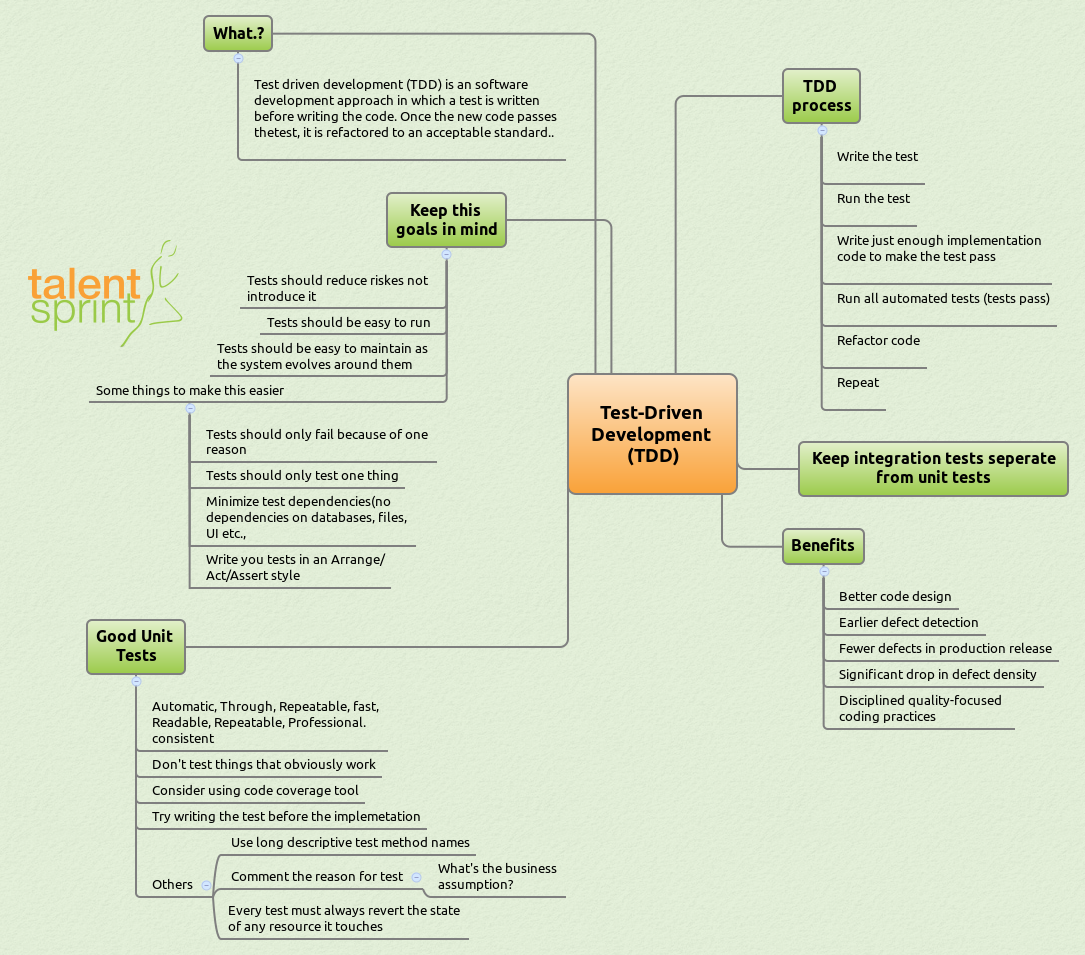
\includegraphics[angle=90,height=20cm, width=13cm]{TDD-MM.png}
 \end{center}
 \end{figure}
\begin{figure}[H]
\begin{center}
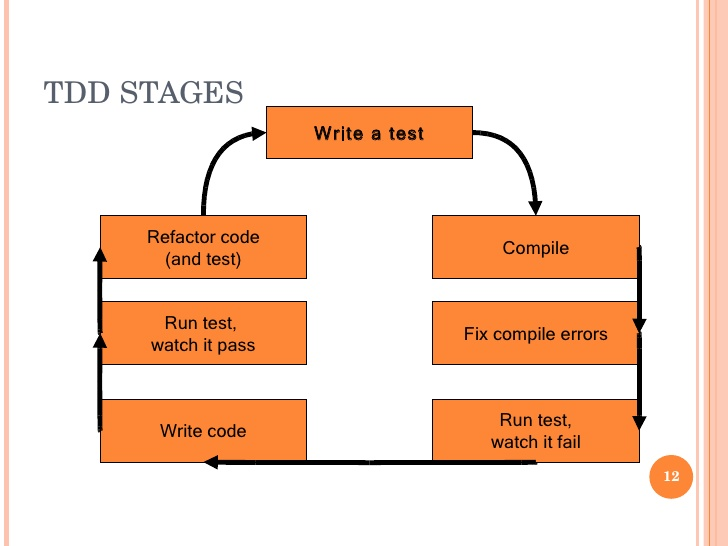
\includegraphics[scale=0.45]{test-driven-development-stages.jpg}
%\caption{Output}
\end{center}
\end{figure}

\subsection*{Sample calculator example using TDD}

\emph{\textbf{Requirement:}} Calculator.square() should correctly calculate square value of the integer passed to it.

\emph{\textbf{CalculatorTest}} class calls the \emph{\textbf{Calculator.square()}} to check its implemention

\lstinputlisting{../Code/CalculatorTest.java}

We have written the test without any implementation, now let's run the code.
\begin{figure}[H]
\begin{center}
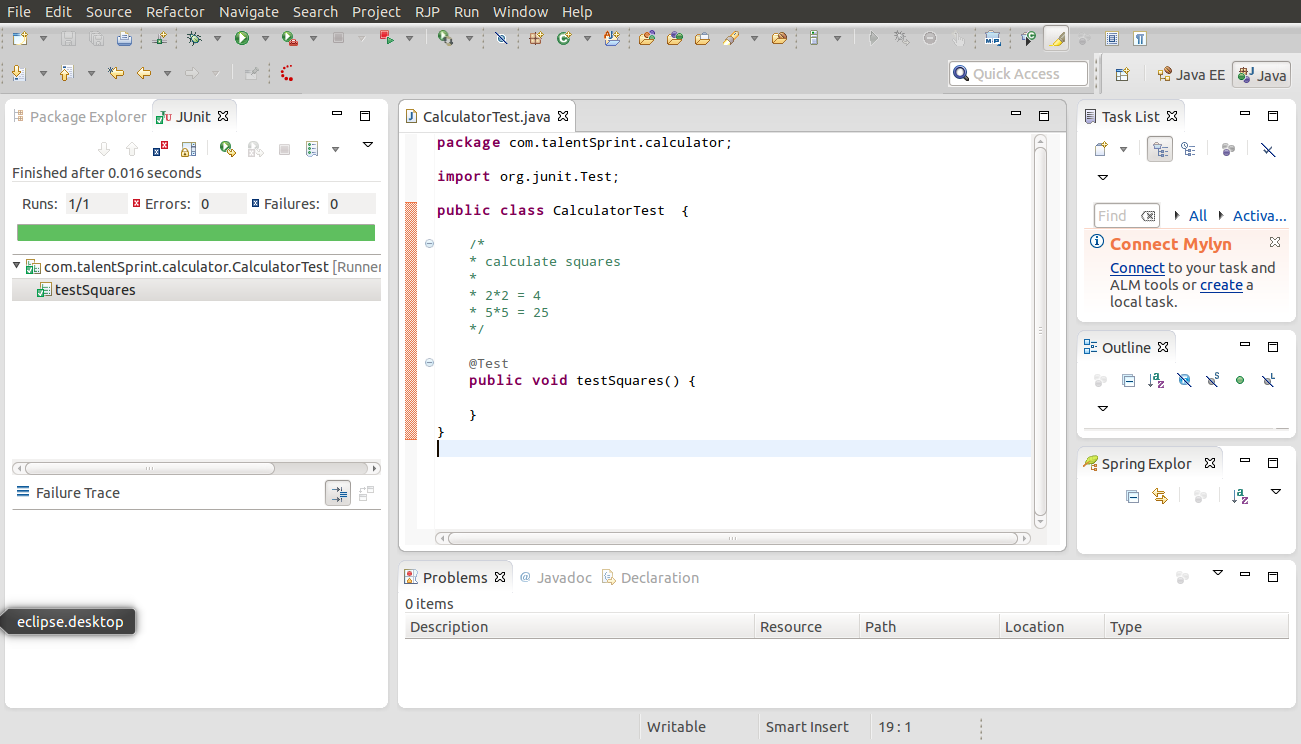
\includegraphics[scale=0.30]{CalculatorTest-1.png}
%\caption{Output}
\end{center}
\end{figure}

The code successfully executed.
Now let's change the implementation for \emph{\textbf{CalculatorTest}} class

\lstinputlisting{../Code/CalculatorTest-1.java}

Code for \emph{\textbf{Calulator.java}}, before logic is implemented to calculate square of an integer

\lstinputlisting{../Code/Calculator.java}

Let's run the unit test again and check the result. The below snapshot shows that the test has failed.
\begin{figure}[H]
\begin{center}
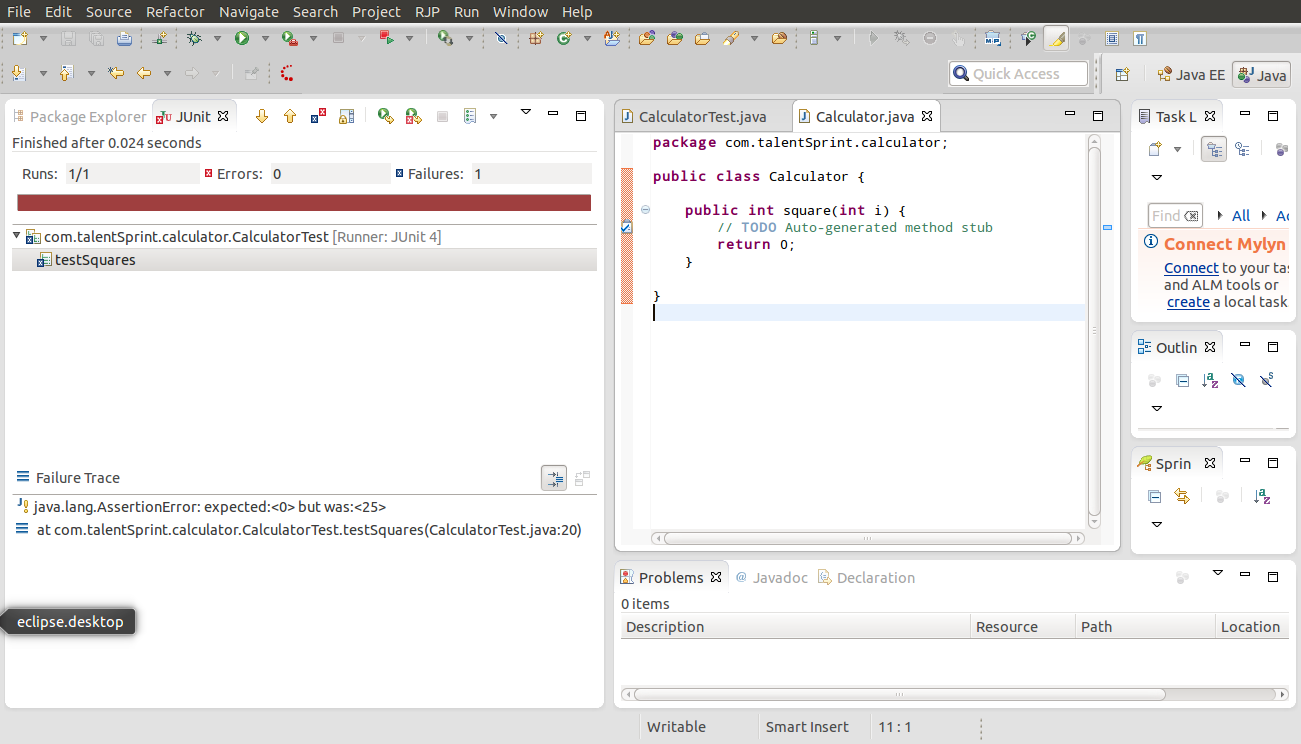
\includegraphics[scale=0.30]{CalculatorTest-2.png}
%\caption{Output}
\end{center}
\end{figure}

\pagebreak
Now let's add the implementation to \emph{\textbf{Calculator}} class.

\lstinputlisting{../Code/CalculatorImpl.java}

Let's rerun the unit test to check the result, the test passed because the expected value is 25 and the returned value is 25

\begin{figure}[H]
\begin{center}
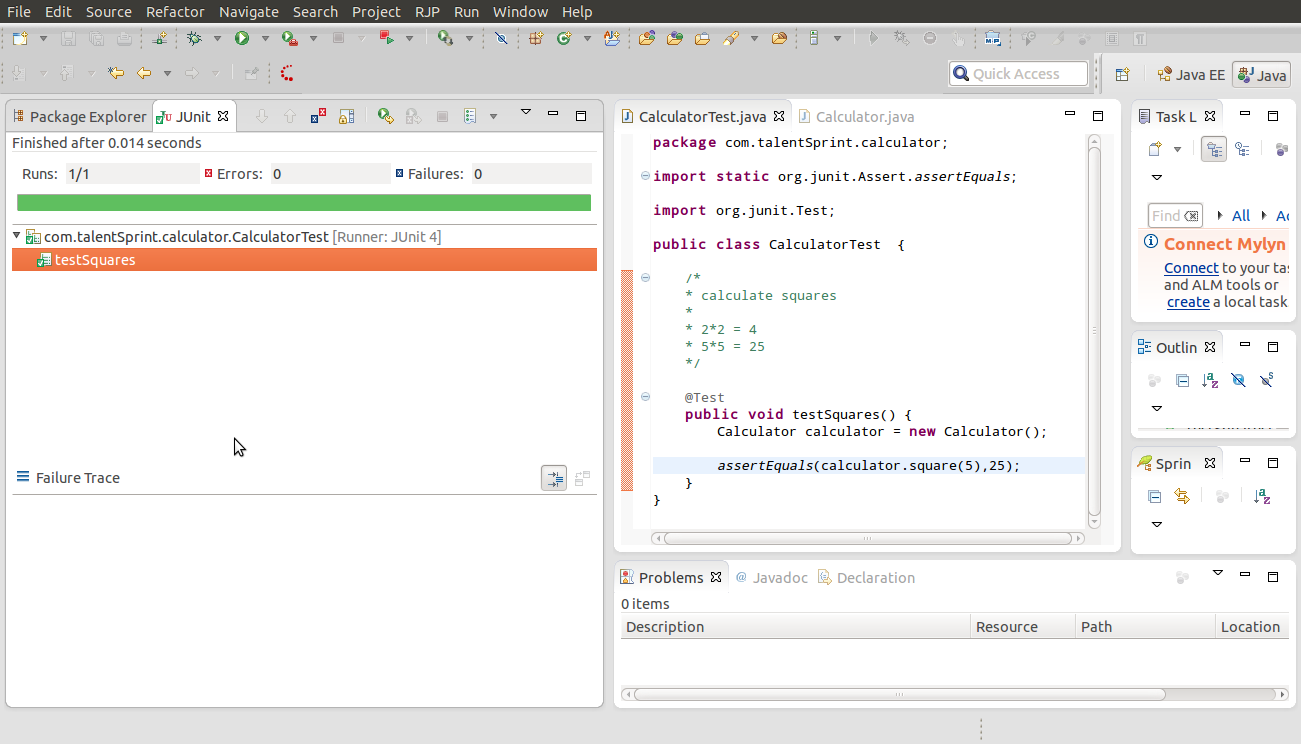
\includegraphics[scale=0.30]{CalculatorTest-3.png}
%\caption{Output}
\end{center}
\end{figure}

\subsection*{Merits of TDD}
The following are generally the Merits of TDD:
\begin{itemize}
\item TDD promotes the development of high quality code.
\item TDD shortens the programming feedback loop.
\item User requirements more easily understood.
\item Reduced software defect rates.
\item Less debug time.
\item TDD provides concrete evidence that your software works.
\end{itemize}

\subsection*{Challenges of TDD}
The following are generally the drawbacks of Traditional testing:
\begin{itemize}
\item Programmers like to code, not to test.
\item Test writing is time consuming.
\item Lot of test code is created and has to be maintained at a significant cost
\item Implement just enough code to get the test to pass.
\end{itemize}

\section*{JUnit}
JUnit promotes the idea of ``first testing then coding'', which emphasis on setting up the test data fora piece of code which can be tested first and then can be implemented. This approach is like ``test a little, code a little, test a little, code a little...'' which increases programmer productivity and stability
of program code that reduces programmer stress and the time spent on debugging.

\subsection*{Features}
\begin{itemize}
\item JUnit is an open source framework, used for writing and running tests.
\item Provides Annotation to identify the test methods.
\item JUnit tests allow you to write code faster which increasing quality.
\item JUnit is elegantly simple. It is less complex and takes less time.
\item JUnit tests can be run automatically and they check their own results and provide immediate feedback. There's no need to manually comb through a report of test results.
\item JUnit tests can be organized into test suites containing test cases and even other test suites.
\item Junit shows test progress in a bar that is green if test is going fine and it turns red when a test fails.
\end{itemize}

\subsection*{What is a Unit Test Case ?}
A Unit Test Case is a part of code which ensures that the another part of code (method) works as expected. To achieve those desired results quickly, test framework is required. JUnit is perfect unit test framework for java programming language.

A formal written test-case is characterized by a known input and by an expected output, which is worked out before the test is executed. The known input should test a precondition and the expected output should test a post condition.
There must be at least two test cases for each requirement: one positive test and one negative test. If a requirement has sub-requirements, each sub-requirement must have at least two test cases as positive and negative.

\subsection*{JUnit Test Framework}
JUnit is a Regression Testing Framework used by developers to implement unit testing in Java and accelerate programming speed and increase the quality of code. JUnit Framework can be easily integrated with either of the followings:
\begin{itemize}
\item Eclipse
\item Ant
\item Maven
\end{itemize}

\subsection*{Features of JUnit Test Framework}
JUnit test framework provides following important features
\begin{itemize}
\item Fixtures
\item Test suites
\item Test runners
\item JUnit classes
\end{itemize}

\subsection*{Fixtures}

\emph{\textbf{Fixtures}} is a fixed state of a set of objects used as a baseline for running tests. The purpose of a test fixture is to ensure that there is a well known and fixed environment in which tests are run so that results are repeatable. It includes
\begin{itemize}
\item setUp() method which runs before every test invocation.
\item tearDown() method which runs after every test method.
\end{itemize}
Example:

\lstinputlisting{../Code/JavaTest.java}

\subsection*{Test suite}
\emph{\textbf{Test suite}} means bundle a few unit test cases and run it together.

Example:

\lstinputlisting{../Code/JunitTestSuite.java}

\lstinputlisting{../Code/TestJunit1.java}

\lstinputlisting{../Code/TestJunit2.java}


\subsection*{Test runner}
\emph{\textbf{Test runner}} is used for executing the test cases. Here is an example which assumes TestJunit test class already exists.

\lstinputlisting{../Code/TestRunner.java}

\subsection*{JUnit classes}
JUnit classes are important classes which is used in writing and testing JUnits. Some of the important classes are

\begin{itemize}
\item \emph{\textbf{Assert}} which contain a set of assert methods.
\item \emph{\textbf{TestCase}} which contain a test case defines the fixture to run multiple tests.
\item \emph{\textbf{TestResult}} which contain methods to collect the results of executing a test case.
\item \emph{\textbf{TestSuite}} A TestSuite is a Composite of Tests.
\end{itemize}

\subsection*{Annotation}
Annotations are like meta-tags that you can add to you code and apply them to methods or in class. These annotation in JUnit gives us information about test methods, which methods are going to run before and after test methods, which methods run before and after all the methods, which methods or class will be ignore during execution. List of annotations and their meaning in JUnit

\begin{itemize}
\item \emph{\textbf{@Test}} - The Test annotation tells JUnit that the public void method to which it is attached can be run as a test case.
\item \emph{\textbf{@Before}} - Annotating a public void method with @Before causes that method to be run before each Test method.
\item \emph{\textbf{@After}} - Annotating a public void method with @After causes that method to be run after the Test method.
\item \emph{\textbf{@BeforeClass}} - Annotating a public static void method with @BeforeClass causes it to be run once before any of the test methods in the class.
\item \emph{\textbf{@AfterClass}} - This will perform the method after all tests have finished. This can be used to perform clean-up activities.
\item \emph{\textbf{@Ignore}} - The Ignore annotation is used to ignore the test and that test will not be executed.
\end{itemize}

\subsection*{JUnit Sample example}
Now let's go through a step by step process to get a kick start in JUnit using a basic example.

Create a Class \emph{\textbf{MessageUtil.java}}

\lstinputlisting{../Code/MessageUtil.java}

\emph{\textbf{Create Test Case Class}}
\begin{itemize}
\item Create a java test class say TestJunit.java.
\item Add a test method testPrintMessage() to your test class.
\item Add an Annotaion @Test to method testPrintMessage().
\item Implement the test condition and check the condition using assertEquals API of Junit.
\end{itemize}

\break
Create a java class file name \emph{\textbf{TestJunit.java}}

\lstinputlisting{../Code/TestJunit.java}

\emph{\textbf{Create Test Runner Class}}

\begin{itemize}
\item Create a TestRunner java class.
\item Use runClasses method of JUnitCore class of JUnit to run test case of above created test class.
\item Get the result of test cases run in Result Object.
\item Get failure(s) using getFailures() methods of Result object.
\item Get Success result using wasSuccessful() methods of Result object.
\end{itemize}
Create a java class file name TestRunner.java

\lstinputlisting{../Code/TestRunner.java}

Compile the MessageUtil, Test case and Test Runner classes using javac
Now run the Test Runner which will run test case defined in provided Test Case class.

Verify the output.
It should return

\begin{lstlisting}[numbers=none]
Hello World
true
\end{lstlisting}
Now update TestJunit in so that test fails. Change the message string.
\lstinputlisting{../Code/TestJunit-1.java}

Now run the Test Runner which will run test case defined in provided Test Case class.
Verify the output
\begin{lstlisting}[numbers=none]
Hello World
testPrintMessage(TestJunit): expected: <[New Wor]d> but was: <[Hello Worl]d>
false
\end{lstlisting}

\subsection*{JUnit Exception Test}
Junit provides a handy option of Timeout. If a test case takes more time than specified numberof milliseconds then Junit will automatically mark it as failed. The timeout parameter is used alongwith @Test annotation. Now let's see @Test(expected) in action.

\emph{\textbf{Create a Class}}
\begin{itemize}
\item Create a java class to be tested say \emph{\textbf{MessageUtil.java.}}
\item Add a error condition inside printMessage() method.
\item Add expected exception ArithmeticException to testPrintMessage() test case.
\end{itemize}

\lstinputlisting{../Code/MessageUtilExceptionTest.java}


\emph{\textbf{Create Test Case Class}}
\begin{itemize}
\item Create a java test class say \emph{\textbf{TestJunit.java.}}
\end{itemize}

\lstinputlisting{../Code/TestJunitExceptionTest.java}

\emph{\textbf{Create Test Runner Class}}
\begin{itemize}
\item Create a java class file name \emph{\textbf{TestRunner.java.}}
\end{itemize}

\lstinputlisting{../Code/TestRunner.java}

Compile the MessageUtil, Test case and Test Runner classes using \texttt{javac}

Now run the Test Runner which will run test cases defined in provided Test Case class.

Verify the output. testPrintMessage() test case will be passed.

\begin{lstlisting}[numbers=none]
Inside testPrintMessage()
Robert
Inside testSalutationMessage()
Hi!Robert
true
\end{lstlisting}

Now replace expected exception as IndexOutOfBoundsException in MessageUtil.testPrintMessage() test case and rerun the unit test and verify the output

\begin{lstlisting}[numbers=none]
Inside testPrintMessage()
Robert
Inside testSalutationMessage()
Hi!Robert
testPrintMessage(TestJunit): Unexpected exception, expected<java.lang.IndexOutOfBoundsException> but was<java.lang.ArithmeticException>
false\emph{}
\end{lstlisting}


\subsection*{JUnit Parameterized Test}
JUnit 4 has introduced a new feature Parameterized tests. Parameterized tests allow developer to run the same test over and over again using different values. There are five steps,that you need to follow to create Parameterized tests


\begin{itemize}
\item Annotate test class with @RunWith(Parameterized.class).
\item Create a public static method annotated with @Parameters that returns a Collection of Objects (as Array) as test data set.
\item Create a public constructor that takes in what is equivalent to one ``row'' of test data.
\item Create an instance variable for each ``column'' of test data.
\item Create your tests case(s) using the instance variables as the source of the test data.
The test case will be invoked once per each row of data.
\end{itemize}


\emph{\textbf{Create a Class}}
\begin{itemize}
\item Create a java class to be tested say \emph{\textbf{PrimeNumberChecker.java.}}
\end{itemize}

\emph{\textbf{Create Parameterized Test Case Class}}
\begin{itemize}
\item Create a java test class say \emph{\textbf{PrimeNumberCheckerTest.java.}}
\end{itemize}

\lstinputlisting{../Code/PrimeNumberCheckerTest.java}

\emph{\textbf{Create Test Runner Class}}
\begin{itemize}
\item Create a java class file name \emph{\textbf{TestRunner.java }}
\end{itemize}

\lstinputlisting{../Code/TestRunnerParameterTest.java}

Compile the PrimeNumberChecker, PrimeNumberCheckerTest and Test Runner classes using javac

Now run the Test Runner which will run test cases defined in provided Test Case class.

Verify the output.
\begin{lstlisting}[numbers=none]
Parameterized Number is : 2
Parameterized Number is : 6
Parameterized Number is : 19
Parameterized Number is : 22
Parameterized Number is : 23
true
\end{lstlisting}


\end{document}